\section{Liste der Parks}
\label{parklist}

Diese View gibt Auskunft über alle Parks, welche sich auf unseren Server befinden. Hier kann man den 
Namen, die durchschnittliche Bewertung und Bilder zu den Parks finden. 

\begin{figure}[H]
    \begin{center}
      \frame{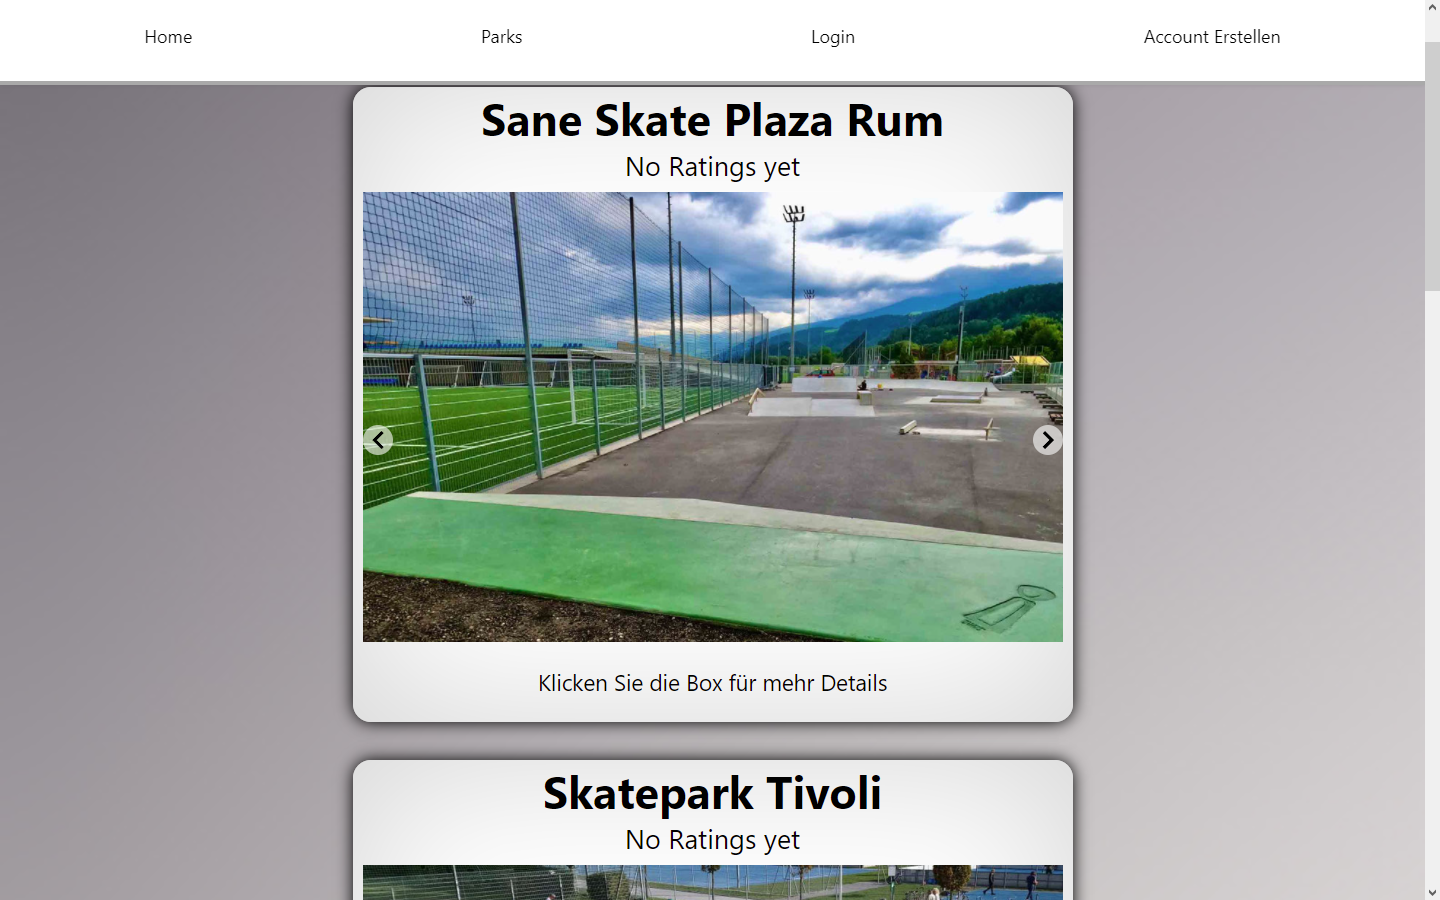
\includegraphics[width=1\textwidth]{Website/Parkliste.png}}
      \caption{Liste der Parks}
    \end{center}
\end{figure}

Hier wurde die selbe \nameref{slideshow} verwendet wie auf der Startseite. Drückt man auf einen der 
Boxen drauf, kommt man auf die \nameref{parkDetails} des Parks, wo man die Bewertungen und Hindernisse,
welche der Park besitzt einsehen kann. 

\subsection{Suchleiste}

Ganz oben auf der Parklisten Ansicht befindet sich eine Suchleiste, mit welche man nach einen bestimmten 
Park suchen kann.

\begin{figure}[H]
    \begin{center}
      \frame{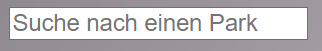
\includegraphics[width=0.5\textwidth]{Website/Suchleiste.png}}
      \caption{Liste der Parks}
    \end{center}
\end{figure}

Wird in die Suchleiste eine Zeichenkette angegeben, werden nur noch die Parks angezeigt, welche diese 
Zeichenkette in ihrem Namen besitzen. Dabei wird Groß- und Kleinschreibung komplett ignoriert um ein 
leichteres Suchen zu ermöglichen. Dafür wird der Input ganz einfach bevor er mit den Namen verglichen wird 
auf Kleinbuchstaben umgeändert.


Ist ein Benutzer eingeloggt, befindet sich über der Suchleiste ein Knopf bei welchen man \nameref{vorschläge}
kann.